% !!!!!!!!!!!!!!!!!!   ВНИМАНИЕ !!!!!!!!!!!!!!!!!!!!!!!!!!!!!!!!!!!!!!!!!!!!!!!!!!!!!!!!!
% Заголовки разделов формируются при помощи команд \section{}, \subsection{}, \subsubsection{}
% Не используйте уровень вложенности заголовков больше трех!
% -----------------------------
% Для оформления теорем, лемм, следствий используйте окружения 
% Def     - Определение
% Teor    - Теорема
% Lem     - Лемма
% Predl   - Предложение
% Ass     - Утверждение
% Cor     - Следствие
% Example - Пример
% -----------------------------
% Доказательство теоремы начинается командой \proof и завершается командой \endproof
% -----------------------------
% Литература помещается в окружение biblio.

\documentclass[11pt, oneside, a4paper]{article}
%\usepackage[cp1251]{inputenc} % кодировка
\usepackage[utf8]{inputenc} % кодировка
\usepackage[english, russian]{babel} % Русские и английские переносы
\usepackage{graphicx}          % для включения графических изображений
\usepackage{cite}              % для корректного оформления литературы
\usepackage{enumitem}
\usepackage{amsmath,amsthm,amssymb}
\usepackage{mathtext}


%стилевой пакет
\usepackage{schoolseminar2020}                                


%\renewcommand{\thefootnote}{*}\footnote{Работа выполнена при частичной финансовой поддержке .....}

\begin{document}
% \udk     - универсальный десятичный классификатор
% \msc     - Индекс предметной классификации (Mathematics Subject Classification)
% \title   - название статьи
% \authors - список авторов
\setcounter{page}{1}


\udk{519.853.4}

\title{
%Способ учета наличия разрывов в задачах многоэкстремальной оптимизации 
Решение задач глобальной оптимизации с учетом возможных разрывов целевой функции
\footnote{Исследование выполнено при финансовой поддержке РФФИ в рамках научного проекта № 19-07-00242.}
}


\authors{К.А. Баркалов, М.А. Усова}
\organizations{Нижегородский государственный университет им. Н.И. Лобачевского}


% \section{название} - заголовок раздела первого уровня
% \subsection{название} - заголовок раздела второго уровня
% \subsubsection{название} - заголовок раздела третьего уровня

\bigskip

В работе рассматривается задача поиска глобального минимума $x^*$ одномерной функции $\varphi(x)$ вида
\begin{equation}\label{problem}
\varphi(x^*)=\min\left\{\varphi(x):x\in\left[a,b\right]\right\}.
\end{equation}
Предполагается, что целевая функция является многоэкстремальной и задана в виде ``черного ящика'', т.е. некоторого алгоритма вычисления значения функции в зависимости от параметра. При этом каждое \textit{испытание} (т.е. вычисление значения функции в области поиска) является трудоемкой операцией.  

Задачи одномерной оптимизации играют важную роль, т.к. многие подходы к решению многомерных задач оптимизации так или иначе основаны на сведении решения исходной многомерной задачи к решению серии связанных задач одномерной оптимизации (см., например, \cite{Grishagin2007,Sergeyev2008}).
В литературе описаны различные методы решения задачи (\ref{problem}) в зависимости от предположений о свойствах целевой функции. Одним из подобных предположений, которое часто выполняется в прикладных оптимизационных задачах, является предположение о том, что целевая функция $\varphi(x)$ удовлетворяет условию Липшица с априори неизвестной константой $L$
\[
\left|\varphi(x')-\varphi(x'')\right|\leq L\left|x'-x''\right|,\; x',x'' \in [a,b],\; 0<L<\infty.
\]
Использование данного свойства целевой функции является типичным для многих подходов к разработке алгоритмов многоэкстремальной оптимизации \cite{Evtushenko2009,Elsakov}. 

Однако в некоторых прикладных задачах свойство липшицевости может не выполняться в силу наличия скачкообразных изменений значений функции в ряде точек области поиска. Мы будем интерпретировать подобные резкие изменения как разрывы первого рода. Иногда множество точек, в которых характеристики объекта претерпевают скачок, известно заранее. Вместе с тем существуют задачи, в которых нет априорных оценок точек разрыва, но есть информация, что такие точки возможны.

Известные методы решения подобных задач, как правило, либо обобщают понятие градиента для разрывных функций \cite{Batuhtin1997}, либо принадлежат классу биоинспирированных алгоритмов \cite{Jihui}. Указанные методы обеспечивают, вообще говоря, поиск только \textit{локального решения} задачи. 

В докладе на конференции будет представлен разработанный в ННГУ им. Н.И. Лобачевского эффективный алгоритм для поиска \textit{глобального решения} многоэкстремальных задач с разрывными функциями. 
Данный алгоритм является дальнейшим развитием \textit{алгоритма глобального поиска}, описание, теория сходимости и различные модификации которого представлены в \cite{Strongin2013}. 

В новом алгоритме глобального поиска для разрывных функций (АГП-Р) учет разрывов целевой функции происходит явно, т.е. без операции сглаживания разрыва. 
При этом охватываются случаи как заданных, так и не заданных точек разрыва: при отсутствии информации о координатах точек разрыва их оценка проводится адаптивно, на основе вычисленных значений функции в точках проведенных испытаний.  
Ошибочное определение некоторых точек разрыва не приводит к потере сходимости метода. Решающие правила алгоритма интерпретируют такие точки как случай устранимого разрыва, поскольку левый и правый пределы оптимизируемой функции в таких точках совпадают.

%Более подробный комментарий?


В качестве примера рассмотрим задачу минимизации функции
\begin{equation}\label{test}
\varphi(x) = 0.1 \sum_{i=1}^5{i\sin(10(i+1)x+i)}+
\begin{cases}
	-4,  &0   \leq x < 3.1\\
	10,  &3.1 \leq x < 4.6\\
	 0,  &4.6 \leq x < 7.0\\
	30,  &7.0 \leq x < 9.0\\
	 0,  &9.0 \leq x \leq 10.0
\end{cases}
\end{equation}
при $x\in[0,10]$. 

Для решения задачи использовался алгоритм глобального поиска для разрывных функций (АГП-Р), точность поиска решения была выбрана $\epsilon = 0.001$. На рис. \ref{ris1} изображен график функции, на котором наглядно видны точки разрывов. 
Штрихами под графиком обозначены точки поисковых испытаний, потребовавшихся алгоритму для решения задачи с указанной точностью. 
В случае, когда точки разрывов были известны, метод провел XXX испытаний (штрихи верхнего ряда). В случае, когда точки разрывов не были заданы заранее и идентифицировались в процессе поиска, методу потребовалось YYY испытаний (штрихи нижнего ряда). В обоих случаях распределение точек испытаний показывает наличие сходимости лишь к глобальному экстремуму, накопления точек около локальных экстремумов --- отсутствуют.

\begin{figure}%[!ht]
	\begin{center}
			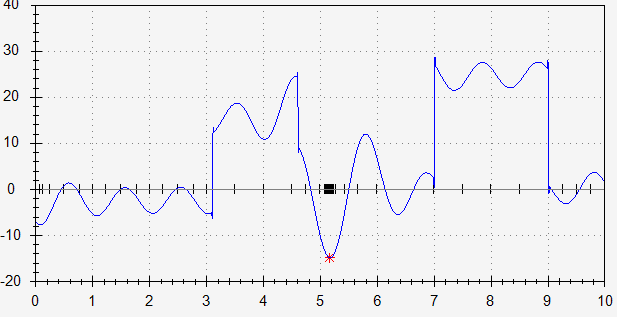
\includegraphics[width=0.7\linewidth]{ris1.png}
			\caption{График разрывной целевой функции и точки испытаний} %% подпись к рисунку
      \label{ris1}
	\end{center}
\end{figure}


Для демонстрации эффективности алгоритма глобального поиска для разрывных функций (АГП-Р), проведем его сравнение с алгоритмом имитации отжига (ИО), реализованным в MATLAB Global Optimization Toolbox. В качестве основного критерия сравнения будем использовать число поисковых испытаний (т.е. вычислений значений целевой функции), выполненное методом до достижения сходимости. 

Сравнение алгоритмов проводилось при решении 100 задач с разрывной целевой функцией, которые были построены аналогично задаче (\ref{test}). В таблице 1 представлено число решенных задач и среднее число испытаний, выполненных методами при решении серии. Задача считалась решенной, если для точки некоторого испытания $x^k$ выполнялось условие $\left|x^k-x^*\right|\leq \delta$, где $x^*$ --- известное решение задачи, а $\delta = 10^{-2}$. При этом точность, используемая в условии остановки методов, была выбрана на порядок меньшей, $\epsilon=10^{-3}$.

\begin{table}[h]
	\caption{Результаты решения серии задач с разрывными функциями}
	\begin{center}
		\begin{tabular}{|c|c|c|}
			\hline
			Метод & Решено задач & Среднее число испытаний \\
			\hline
			\hline
			ИО    &  89 &   876  \\
			\hline
			АГП-Р & 100  & 81 \\
			\hline
		\end{tabular}
	\end{center}
\end{table}

Результаты показывают, что метод АГП-Р успешно решил все задачи серии, тогда как метод имитации отжига не справился с решением 11 задач, затратив при этом в среднем в 10 раз больше испытаний.


\begin{biblio}

%\bibitem{fio_bib1} Шаманаев П. А., Язовцева О. С. Достаточные условия локальной покомпонентной асимптотической эквивалентности нелинейных систем обыкновенных дифференциальных уравнений и ее приложение к устойчивости по части переменных // Журнал Средневолжского математического общества. 2017. Т. 19, № 1. С. 102--115.

%\bibitem{fio_bib2} Шаманаев П. А., Язовцева О. С. Достаточные условия полиустойчивости по части переменных нулевого решения нелинейных систем обыкновенных дифференциальных уравнений // Журнал Средневолжского математического общества.  2018. Т. 20, № 3. С. 304--317.

%\bibitem{fio_bib3} Шаманаев П. А., Язовцева О. С. Исследование устойчивости положения равновесия системы динамики биоценоза в условиях межвидового взаимодействия // Вестник Мордовского университета. 2018. Т. 28, № 3. С. 321–332.

%\bibitem{fio_bib4} Малкин И. Г. Теория устойчивости движения. М.: Наука, 1966. 533 с.



\bibitem{Grishagin2007} 
Городецкий~С.Ю., Гришагин~В.А. Нелинейное программирование и многоэкстремальная оптимизация. Н.~Новгород: Изд-во ННГУ, 2007. 489~с.

\bibitem{Sergeyev2008}
Сергеев Я.Д., Квасов Д.Е. Диагональные методы глобальной оптимизации. М.: Физматлит, 2008. 352 с. 

\bibitem{Evtushenko2009}
Евтушенко Ю.Г., Малкова В.У., Станевичюс А.-И.А. Параллельный поиск глобального экстремума функций многих переменных // Ж. вычисл. матем. и матем. физ. 2009. Т. 49, № 2.  С. 255--269.

\bibitem{Elsakov}
Елсаков С.М., Ширяев В.И. Однородные алгоритмы многоэкстремальной оптимизации // Ж. вычисл. матем. и матем. физ. 2010. Т. 50, № 10. С. 1727--1740.

\bibitem{Batuhtin1997}
Батухтин В.Д., Бигильдеев С.И., Бигильдеева Т.Б. Численные методы решения разрывных экстремальных задач // Изв. РАН, сер. теория и сист. управления. 1997. Т. 3. С. 113--120.

\bibitem{Jihui}
Jihui Z., Junqin X. A new differential evolution for discontinuous optimization problems // 
Proceedings of the Third International Conference on Natural Computation. 2007. Vol. 3. P. 483--487.

\bibitem{Strongin2013}
Стронгин Р.Г., Гергель В.П., Гришагин В.А., Баркалов К.А. Параллельные вычисления в задачах глобальной оптимизации. М.: Изд-во МГУ, 2013. 280 с.




\end{biblio}

\msc{90C26}

\title{Solving global optimization problems taking into account possible discontinuities of the objective function}

\authors{K.A. Barkalov, M.A. Usova}
\organizations{ Lobachevsky State University of Nizhni Novgorod }



\end{document}

